

%%% BEGIN CHAPTER 4 CHROMATIN ACCESSIBILITY %%%

\chapter[Genome--wide chromatin accessibility changes reveal \\ influential regulatory factors in ILC progenitor]{Genome--wide chromatin accessibility changes reveal influential regulatory factors in ILC progenitor}

\section{ABSTRACT}

Innate lymphoid cells (ILCs) develop from common precursor downstream of lymphoid progenitors. Restriction of developmental potential to innate lymphoid lineages from the common lymphoid precursor is accompanied by a rich set of changes in transcriptional regulation. By a combination of genome-wide transcriptional and chromatin accessibility profiling, we identify regulatory factors affiliated with early epigenetic features that define the ILC progenitor. Our findings highlight the predominant roles TCF, ROR, GATA, and RUNX family members have in promoting ILC differentiation while elaborating their global appearance patterns in enhancers. 

\section{INTRODUCTION}

Innate lymphoid cells (ILCs) monitor peripheral mucosal tissues and are responsible for rapid cytokine secretion in response to inflammatory signals. As innate effectors, ILCs mediate immunity in the absence of somatically rearranged antigen receptors characteristic of adaptive B and T cells. Interestingly, ILCs have a shared developmental origin with the B and T cell lineages and are derived from the common lymphoid progenitor (CLP) \cite{yang2011,mebius2001}. Following divergence from the adaptive cell fates, CLP are capable of differentiating into three groups of differentiated ILC forms analogous to the three classes of CD4\UP{} T helper (Th) cell subsets in both cytokine production and transcriptional determination \cite{artis2015}. Type 1 ILCs, including conventional natural killer cells (cNKs) and ILC1, produce \IFNg and express the lineage-determining transcription factor Tbx21 (also called T-bet) similar to Th1 cells. ILC2s produce IL5 and IL13 and express the lineage-determining transcription factor Gata3 similar to Th2 cells. Finally, type 3 ILCs, including lymphoid tissue inducer cells (LTi) and a variety of ILC3 cells, produce IL17 and IL22 and express the lineage-determining transcription factor \RORgt. 

In the effort to comprehensively map the developmental branching structure for this diverse set of innate lineages downstream of the CLP, there has been a recent surge in reported ILC progenitor populations with varying degrees of developmental restriction \cite{ishizuka2016review}. In this study, we focus on the innate lymphoid cell precursor (ILCP), a committed ILC progenitor defined by expression of the transcription factor PLZF (encoded by \textit{Zbtb16}) \cite{constantinides2014}. Transfer studies demonstrated that the ILCP efficiently gives rise to all peripheral ILC lineages, ILC1, ILC2 and ILC3, but not LTi, NK, B and T cells. Furthermore, in an in vitro differentiation system, single ILCP progenitors simultaneously gave rise to all three ILC subtypes, confirming a multi-lineage developmental potential. Thus, the ILCP is the farthest downstream ILC progenitor prior to ILC effector differentiation. Accordingly, we are studying the developmental transition of CLP to the ILCP to identify transcriptional and epigenetic changes that specifically define commitment to the common ILC lineage. 

Currently, the studies that define ILC developmental precursors have exclusively characterized gene transcription and protein expression in different ILC developmental stages. Distinct epigenetic landscapes, including DNA and histone modifications as well as chromatin accessibility, found in different cell types effectively contextualize the action of expressed regulatory factors, since non-coding regulatory elements with bound transcription factors can control gene expression from long genomic distances. In this way, analysis of regulatory enhancers can reveal both factors induced downstream of transcriptional regulators as well as regulatory network interactions. Chromatin accessibility profiling of differentiated ILC effector subsets has been used to show that differentiated ILC contain open chromatin at effector cytokines prior to their induction \cite{shih2016}. Additionally, chromatin accessibility profiling of intestinal ILC effectors characterized the degree of versatility in ILC response to diverse microbial environments \cite{gury2016}. While these studies profile differentiated forms of ILCs, systematic study of chromatin regulation during early ILC development has not yet been performed to our knowledge. It is clear that many regulatory factors play important roles during ILC development and that regulatory factor expression is also very dynamic in early ILC specification \cite{ishizuka2016review}. Given that epigenetic information can propagate over longer time-scales than gene expression during development \cite{bornstein2014,lara2014}, by examining chromatin regulation in ILC progenitors we can deepen our understanding of ILC regulatory factor interactions and genome-wide influences. 

Here we present the simultaneous characterization of genome-wide transcription and chromatin accessibility changes that occur during ILC lineage restriction. We identify the comprehensive set of transcriptional changes that define the transition of CLP to ILCP, including several transcription factors with uncharacterized roles in ILC development. Our corresponding genome-wide regulome analysis revealed that many distal regulatory elements are substantially changed during this transition. We performed statistical modeling of transcription factor motif presence in regulatory elements to uncover the transcription factors most strongly associated with particular chromatin dynamics. In addition to regulatory motifs that enrich for opening or closing chromatin, we also found a large number of regulatory motifs that enrich specifically for unchanged chromatin. Our systematic survey of regulatory factors predictive of chromatin dynamics revealed that TCF, ROR, GATA, and RUNX family members are widely impactful regulators during ILC specification. 


\section{RESULTS}

\subsection{Transcriptional changes from CLP to ILCP}

We performed genome-wide RNA sequencing (RNA-Seq) analysis to establish a comprehensive transcriptional characterization of the ILCP. We isolated ILCP (defined as Lin\UM{} Il7r\UP{} \ab\UP{} PLZF\UP{} Cxcr5\UM) and CLP (defined as Lin\UM{} Il7r\UP{} cKit\U{int} Sca-1\U{int} Flt3\U{high}) populations in adult bone marrow extracted from PLZF-GFP reporter mice as previously described \cite{constantinides2014}. Due to the rarity of the ILCP (only thousands of cells per mouse), we could only perform sequencing of a single biological replicate of ILCP. To distinguish substantial changes in transcription, we performed differential expression analysis with a fixed biological coefficient of variation and chose a significance cutoff that yielded 201 upregulated and 164 downregulated genes (see methods for details, Figure \ref{fig:chap4_tran}A).

%% Chapter 4 Figure 1 Transcription Profiles %%
\begin{figure}[h]
\begin{center}
	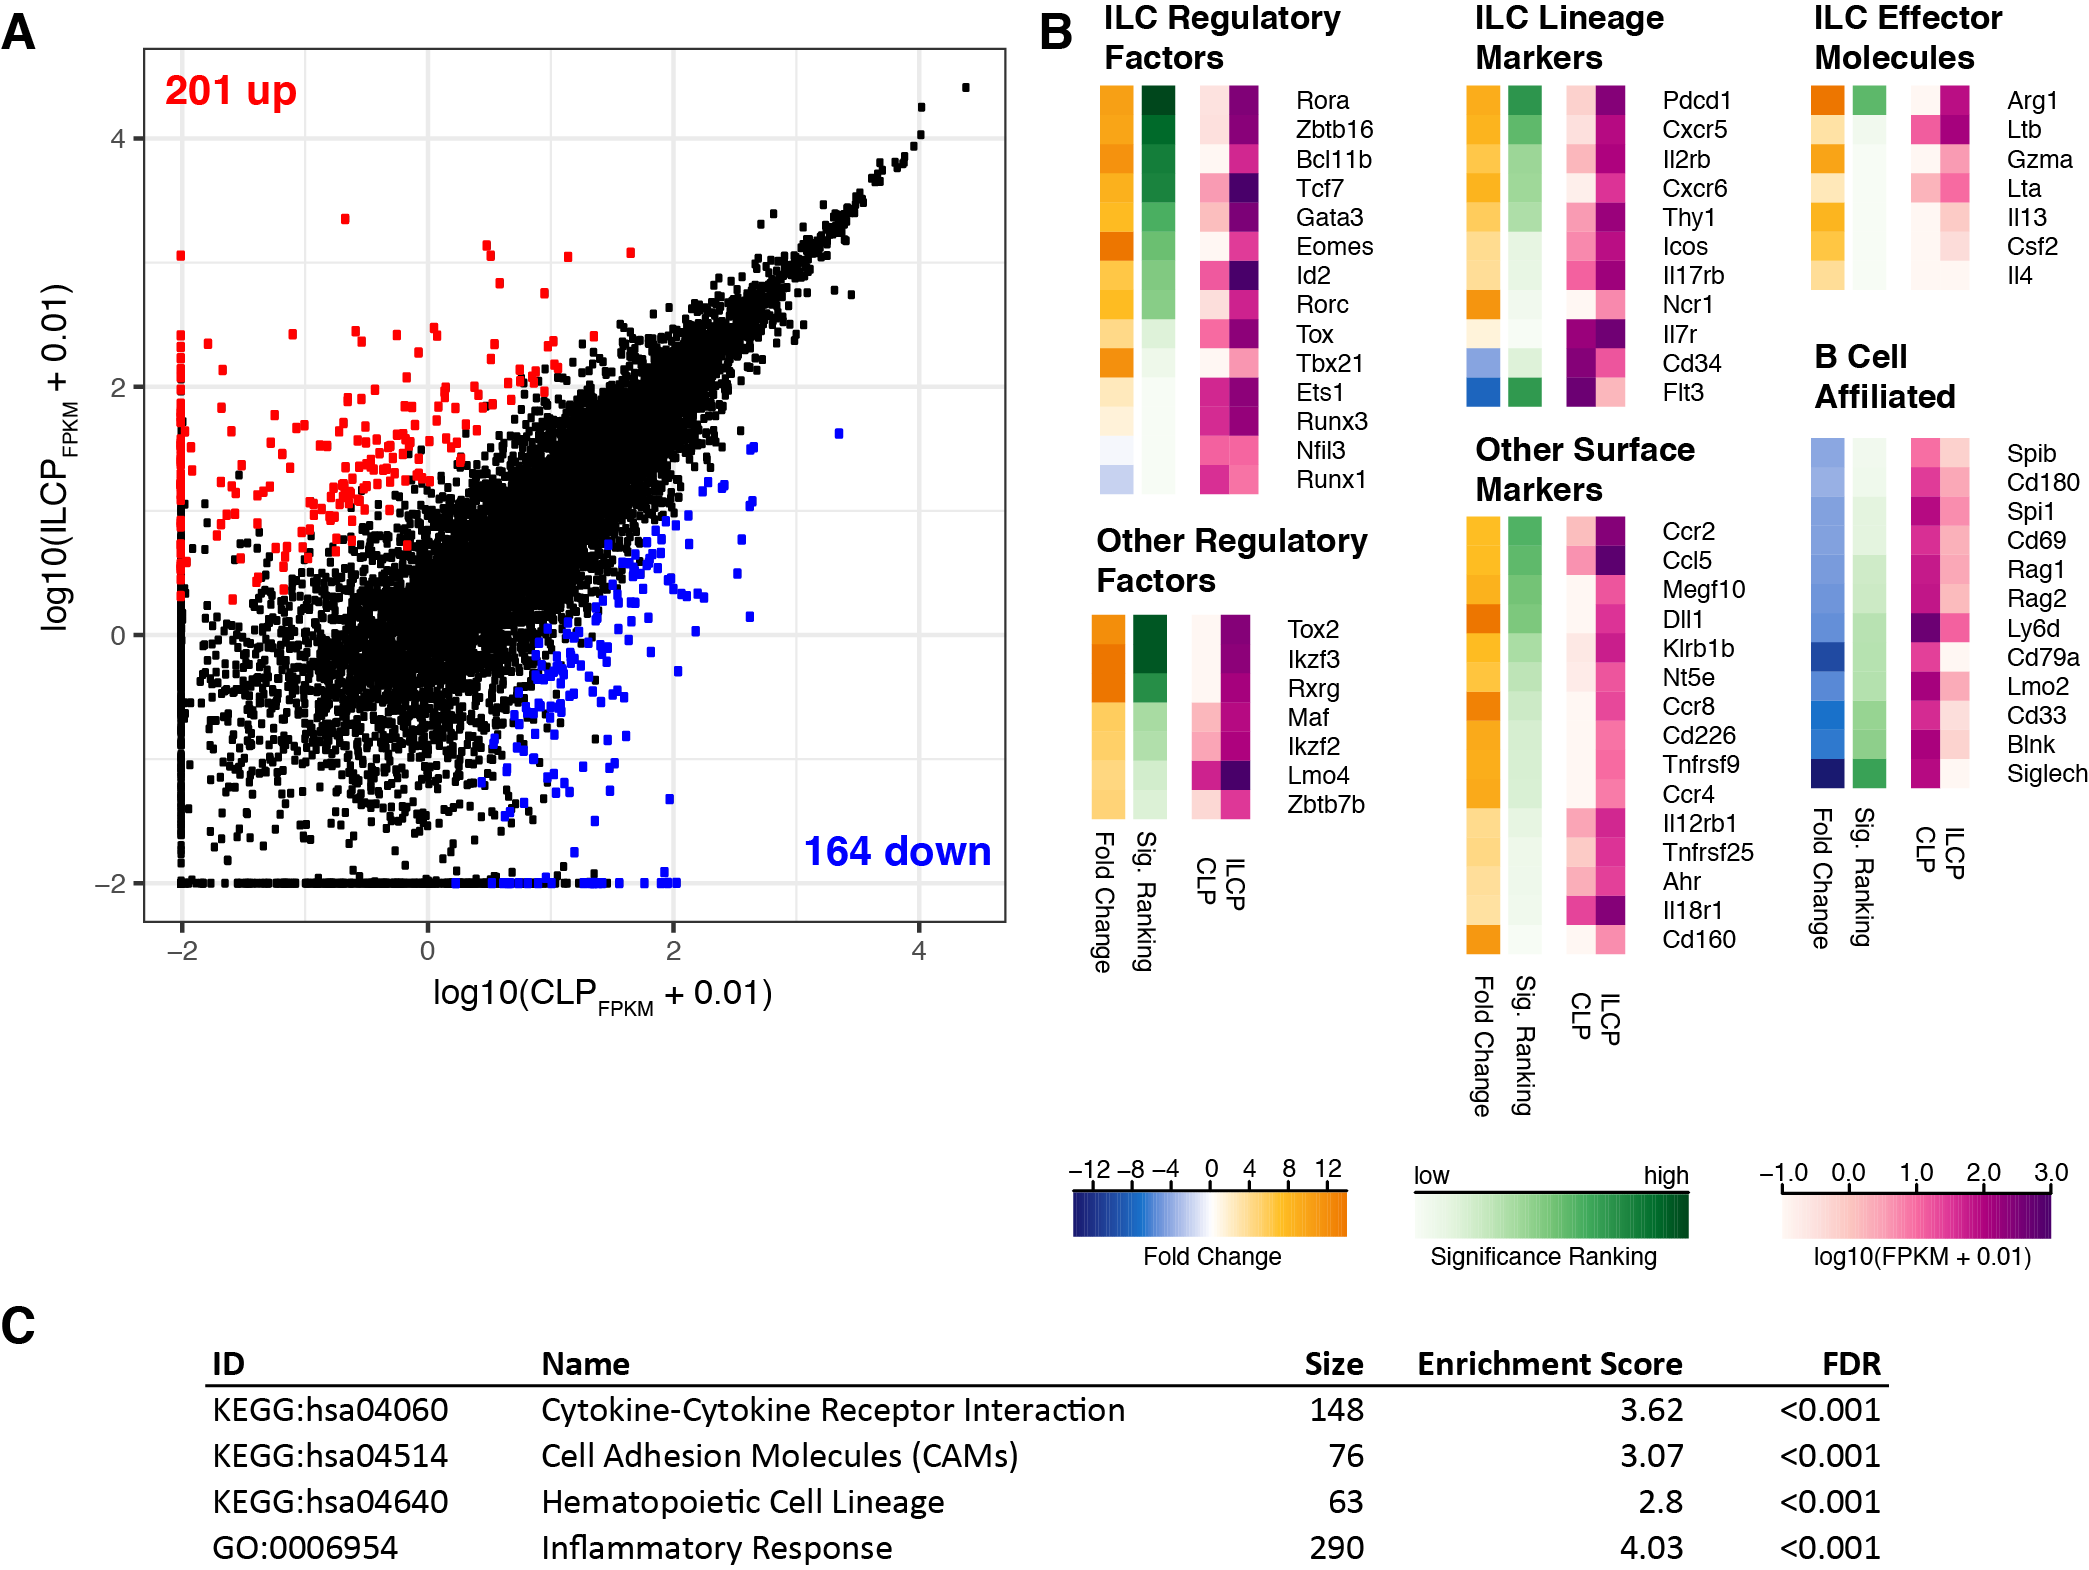
\includegraphics[width=\textwidth]{figures/chapter4/Figure_1_transcription_profiles}
\end{center}
	\caption{Transcriptional changes from CLP to ILCP.} 
	A) Log scale FPKM values in CLP and ILCP. Red, upregulated; blue, downregulated. B) Select transcriptional characterization of CLP and ILCP. C) Top enriched KEGG and GO pathways between CLP and ILCP.
	\label{fig:chap4_tran}
\end{figure}

Despite only affording comparison between single replicates, the derived gene rankings demonstrate the quality of transcriptional profiling (Figure \ref{fig:chap4_tran}B). Many key transcription factors that regulate ILC development appear among the most substantially changing genes, including \textit{Zbtb16} (encoding PLZF), \textit{Tcf7}, \textit{Id2}, \textit{Tox}, \textit{Bcl11b} and \textit{Gata3}. Each of these regulatory factors has been individually shown to be necessary for proper ILC development and each is highly expressed in ILCP. Other key regulators like \textit{Nfil3} and \textit{Runx1} were expressed in both CLP and ILCP but appeared unchanged in the transition from CLP to ILCP. In single-cell transcriptional studies \cite{ishizuka2016}, these factors have transient transcriptional dynamics immediately prior to ILCP state, which were likely averaged out when sequenced in bulk. We also observe substantial upregulation of ILC lineage-specific transcription factors such as \textit{Tbx21}, \textit{Rorc}, and \textit{Rora}. From single-cell profiling, we expect one third of ILCP to be undergoing initial steps of differentiation and so the appearance of these lineage restricted transcription factors likely derive from these differentiating subpopulations.

We found an additional set of transcription factors without well-characterized roles in ILC development, including \textit{Ikzf2}, \textit{Ikzf3}, \textit{Rxrg}, \textit{Maf}, \textit{Lmo4}, \textit{Tox2} and \textit{Zbtb7b}. Two members of the Ikaros family of zinc-finger transcription factors, Ikzf2 and Ikzf3, are substantially upregulated in ILCP. Members of the Ikaros family of transcriptional regulators are widely expressed throughout hematopoiesis and influence a variety of cell-fate decisions \cite{John2011}. Ikzf3, also known as Aiolos, can influence the development and survival of the B cell fate and is one of the most upregulated genes in ILCP. Rxrg appears strongly upregulated in ILCP, though from single-cell investigation we know Rxrg expression is affiliated with the ILC2 lineage \cite{ishizuka2016}. Since Maf also plays important roles in the differentiation of T helper cell subsets \cite{macian2005}, expression of Maf in ILCP could represent an additional shared developmental determinant between the lineages. Many of these transcription factors have appeared consistently in ILC profiling studies \cite{seillet2016,constantinides2015,ishizuka2016,seehus2015}, but whether these factors have precise roles remain to be determined. 

These changes in expression of key regulators coincide with expected changes in surface-expressed lineage markers, including upregulation of \textit{Pdcd1}, \textit{Il7r} and \textit{Thy1} as well as downregulation of \textit{Cd34} and \textit{Flt3}. Additionally, we observe upregulation of many ILC lineage markers, such as \textit{Ncr1}, \textit{Il2rb}, \textit{Icos}, \textit{Il17rb}, \textit{Cxcr5} and \textit{Cxcr6}. The inhibitory receptor Pdcd1 has been recently revealed to coincide with PLZF expression and therefore acts as an effective alternative marker to Zbtb16-GFP for ILC progenitor populations \cite{yu2016}. In our comparison, \textit{Pdcd1} is one of the most strongly upregulated genes in ILCP. Among other immunoregulatory surface-expressed molecules we observed upregulation of interleukin receptors \textit{Il18r1} and \textit{Il12rb1}, \textit{Ccl5}, chemokine receptors \textit{Ccr2}, \textit{Ccr4} and \textit{Ccr8}, tumor necrosis factors \textit{Tnfrsf9} and \textit{Tnfrsf25}, as well as \textit{Ahr}, \textit{Megf10}, \textit{Dll1}, \textit{Klrb1b}, \textit{Nt5e}, \textit{Cd160} and \textit{Cd226}. As the ILCP represents the developmental stage just prior to significant differentiation, we only observe slight upregulation of a few ILC effector cytokines, including \textit{Arg1}, \textit{Gzma}, \textit{Il4}, \textit{Il13}, \textit{Csf2}, \textit{Lta}, and \textit{Ltb}. At this stage, the expression of ILC specific transcription factors are much more substantial that those of effector molecules as expected.

The most substantially downregulated genes in ILCP included many B cell development affiliated factors. The ETS family transcription factors Spi1 (or PU.1) and Spib are required for functional lymphoid lineage priming and B cell differentiation and were much more highly expressed in CLP than in ILCP. The recombination-activating genes Rag1 and Rag2, which are responsible for adaptive antigen receptor rearrangement were also notably downregulated in ILCP. One of the most strongly downregulated genes in ILCP was Blnk, a linker protein in B cell receptor signaling pathways required for complete B cell development \cite{minegishi1999}. We also observed downregulation of B cell associated surface markers, including \textit{Cd180}, \textit{Cd69}, \textit{Cd79a}, \textit{Ly6d} and Siglec family members \textit{Cd33} and \textit{Siglech}. The downregulation of B cell affiliated factors in ILCP was contrasted by the upregulation of a few of genes associated with T cell differentiation, including T cell receptor constant region genes, \textit{Themis}, and T cell signaling genes \textit{Txk} and \textit{Itk}. As these T cell genes are associated with adaptive signaling complexes, it is unlikely they play functional roles in ILCs, and perhaps more likely indicate a low level of sequencing contamination.

Gene set enrichment analysis confirmed that the predominant biological processes being altered are immune-related, as we found cytokine-cytokine receptor interaction, cell adhesion molecules, and hematopoietic cell lineage comprise the three most enriched KEGG pathways while inflammatory response was the most enriched GO pathway (Figure \ref{fig:chap4_tran}C). These transcriptional profiles confirm the relevance of known ILC developmental factors as well as suggest new regulatory factors and markers by global profiling. 


\subsection{Enhanced distal chromatin accessibility during ILC specification}

We further examined the global regulatory landscape during ILC specification by an assay for transposase-accessible chromatin using sequencing (ATAC-seq) \cite{buenrostro2013}. The modest requirements for starting material allowed us to perform this assay with the rare ILC progenitor population isolated ex vivo. To allow direct comparison to transcriptional profiling, we analyzed the transition from CLP (3 replicates) to ILCP (2 replicates). We found ~50,000 total candidate regulatory elements shared among all replicates of either CLP or ILCP. Analysis of differential read-counts revealed 12,367 significantly changing regulatory element peaks between stages, with 6404 upregulated and 5963 downregulated (Figure \ref{fig:chap4_peakloc}A). The greater proportion of ILCP-specific peaks and their larger absolute fold changes illustrates an overall bias towards chromatin opening in ILCP by both peak number and strength. 

%% Chapter 4 Figure 2 Peak Examples %%
\begin{figure}[h]
\begin{center}
	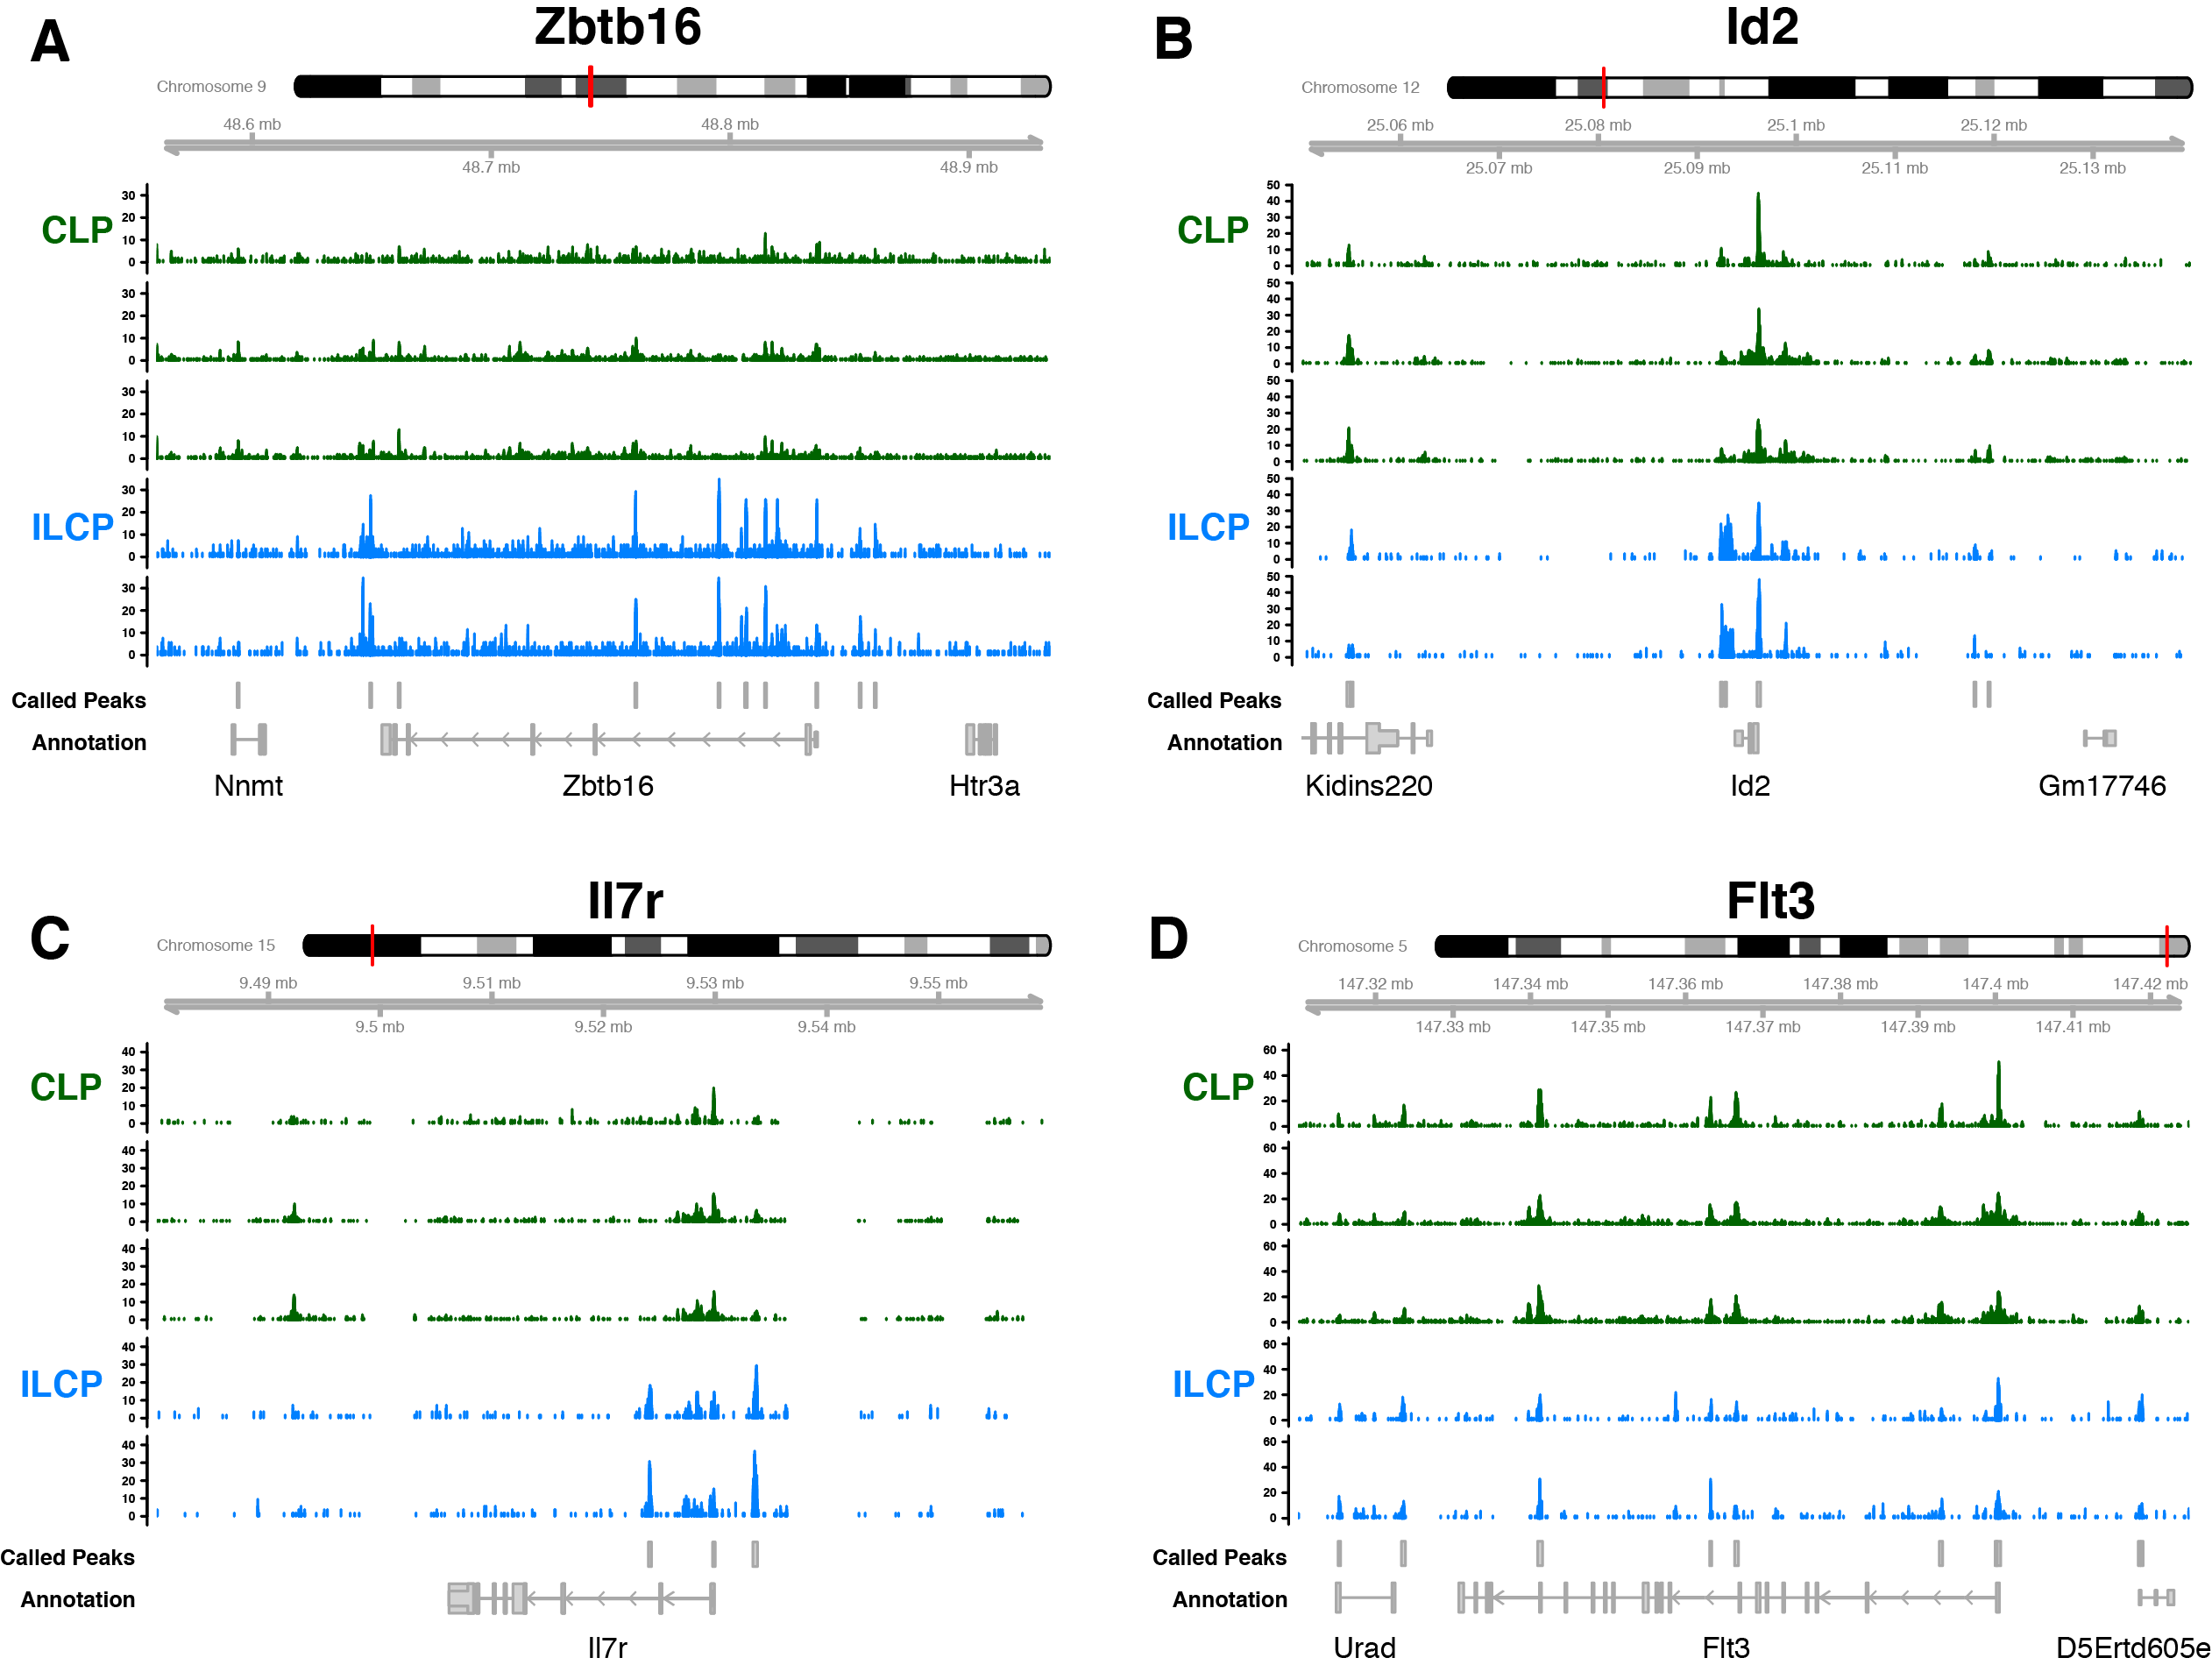
\includegraphics[width=\textwidth]{figures/chapter4/Figure_2_atac_peak_examples}
\end{center}
	\caption{Chromatin accessibility changes from CLP to ILCP.} 
	 ATAC-seq coverage for Zbtb16, Id2, Il7r, and Flt3 in CLP and ILCP samples. Peak features called in either all CLP or all ILCP samples annotated in grey. 
	\label{fig:chap4_peakex}
\end{figure}

We next examined the genomic locations of identified regulatory elements and found an overall enrichment (20-fold) of called peaks in promoter regions ($\pm$1kb of transcription start sites (TSSs)). More specifically, unchanged peaks retained in CLP and ILCP at similar strengths are particularly enriched near gene TSS (Figure \ref{fig:chap4_peakloc}B). Peaks with less than 2 fold change occur more than 30 times expected by chance (Figure \ref{fig:chap4_peakloc}C-D). This location bias suggests that ILC-specific chromatin changes are almost exclusively distal. 

For a few key ILC lineage-associated genes, we observe largely concordant regulation of local chromatin and transcription (Figure \ref{fig:chap4_peakex}). For Zbtb16, many new regulatory elements appear adjacent to the TSS and in a region of $\sim$200kb extending into intronic regions of the gene. A number of regulatory regions adjacent to Id2 have greatly increased openness in ILCP as well. As Zbtb16 and Id2 are strongly upregulated in ILCP, we would expect these ILCP-specific regulatory elements to be responsible for their upregulation in ILCP. Interestingly, while Il7r is already transcribed in CLP, ILCP-specific regulatory elements that appear near the gene TSS accompany more solidified Il7r expression at the ILCP stage. In the other direction, most of the strong regulatory peaks in CLP adjacent to the downregulated marker gene Flt3 have a greatly reduced footprint in ILCP. The general correspondence between chromatin regulation and transcription is not as direct as that illustrated in the aforementioned examples. The presence of discordant regulatory elements even in the aforementioned examples, including reduced peaks near Id2 and Il7r as well as new peaks near Flt3, illustrates the complication. 

%% Chapter 4 Figure 3 Peak Locations %%
\begin{figure}[p]
\begin{center}
	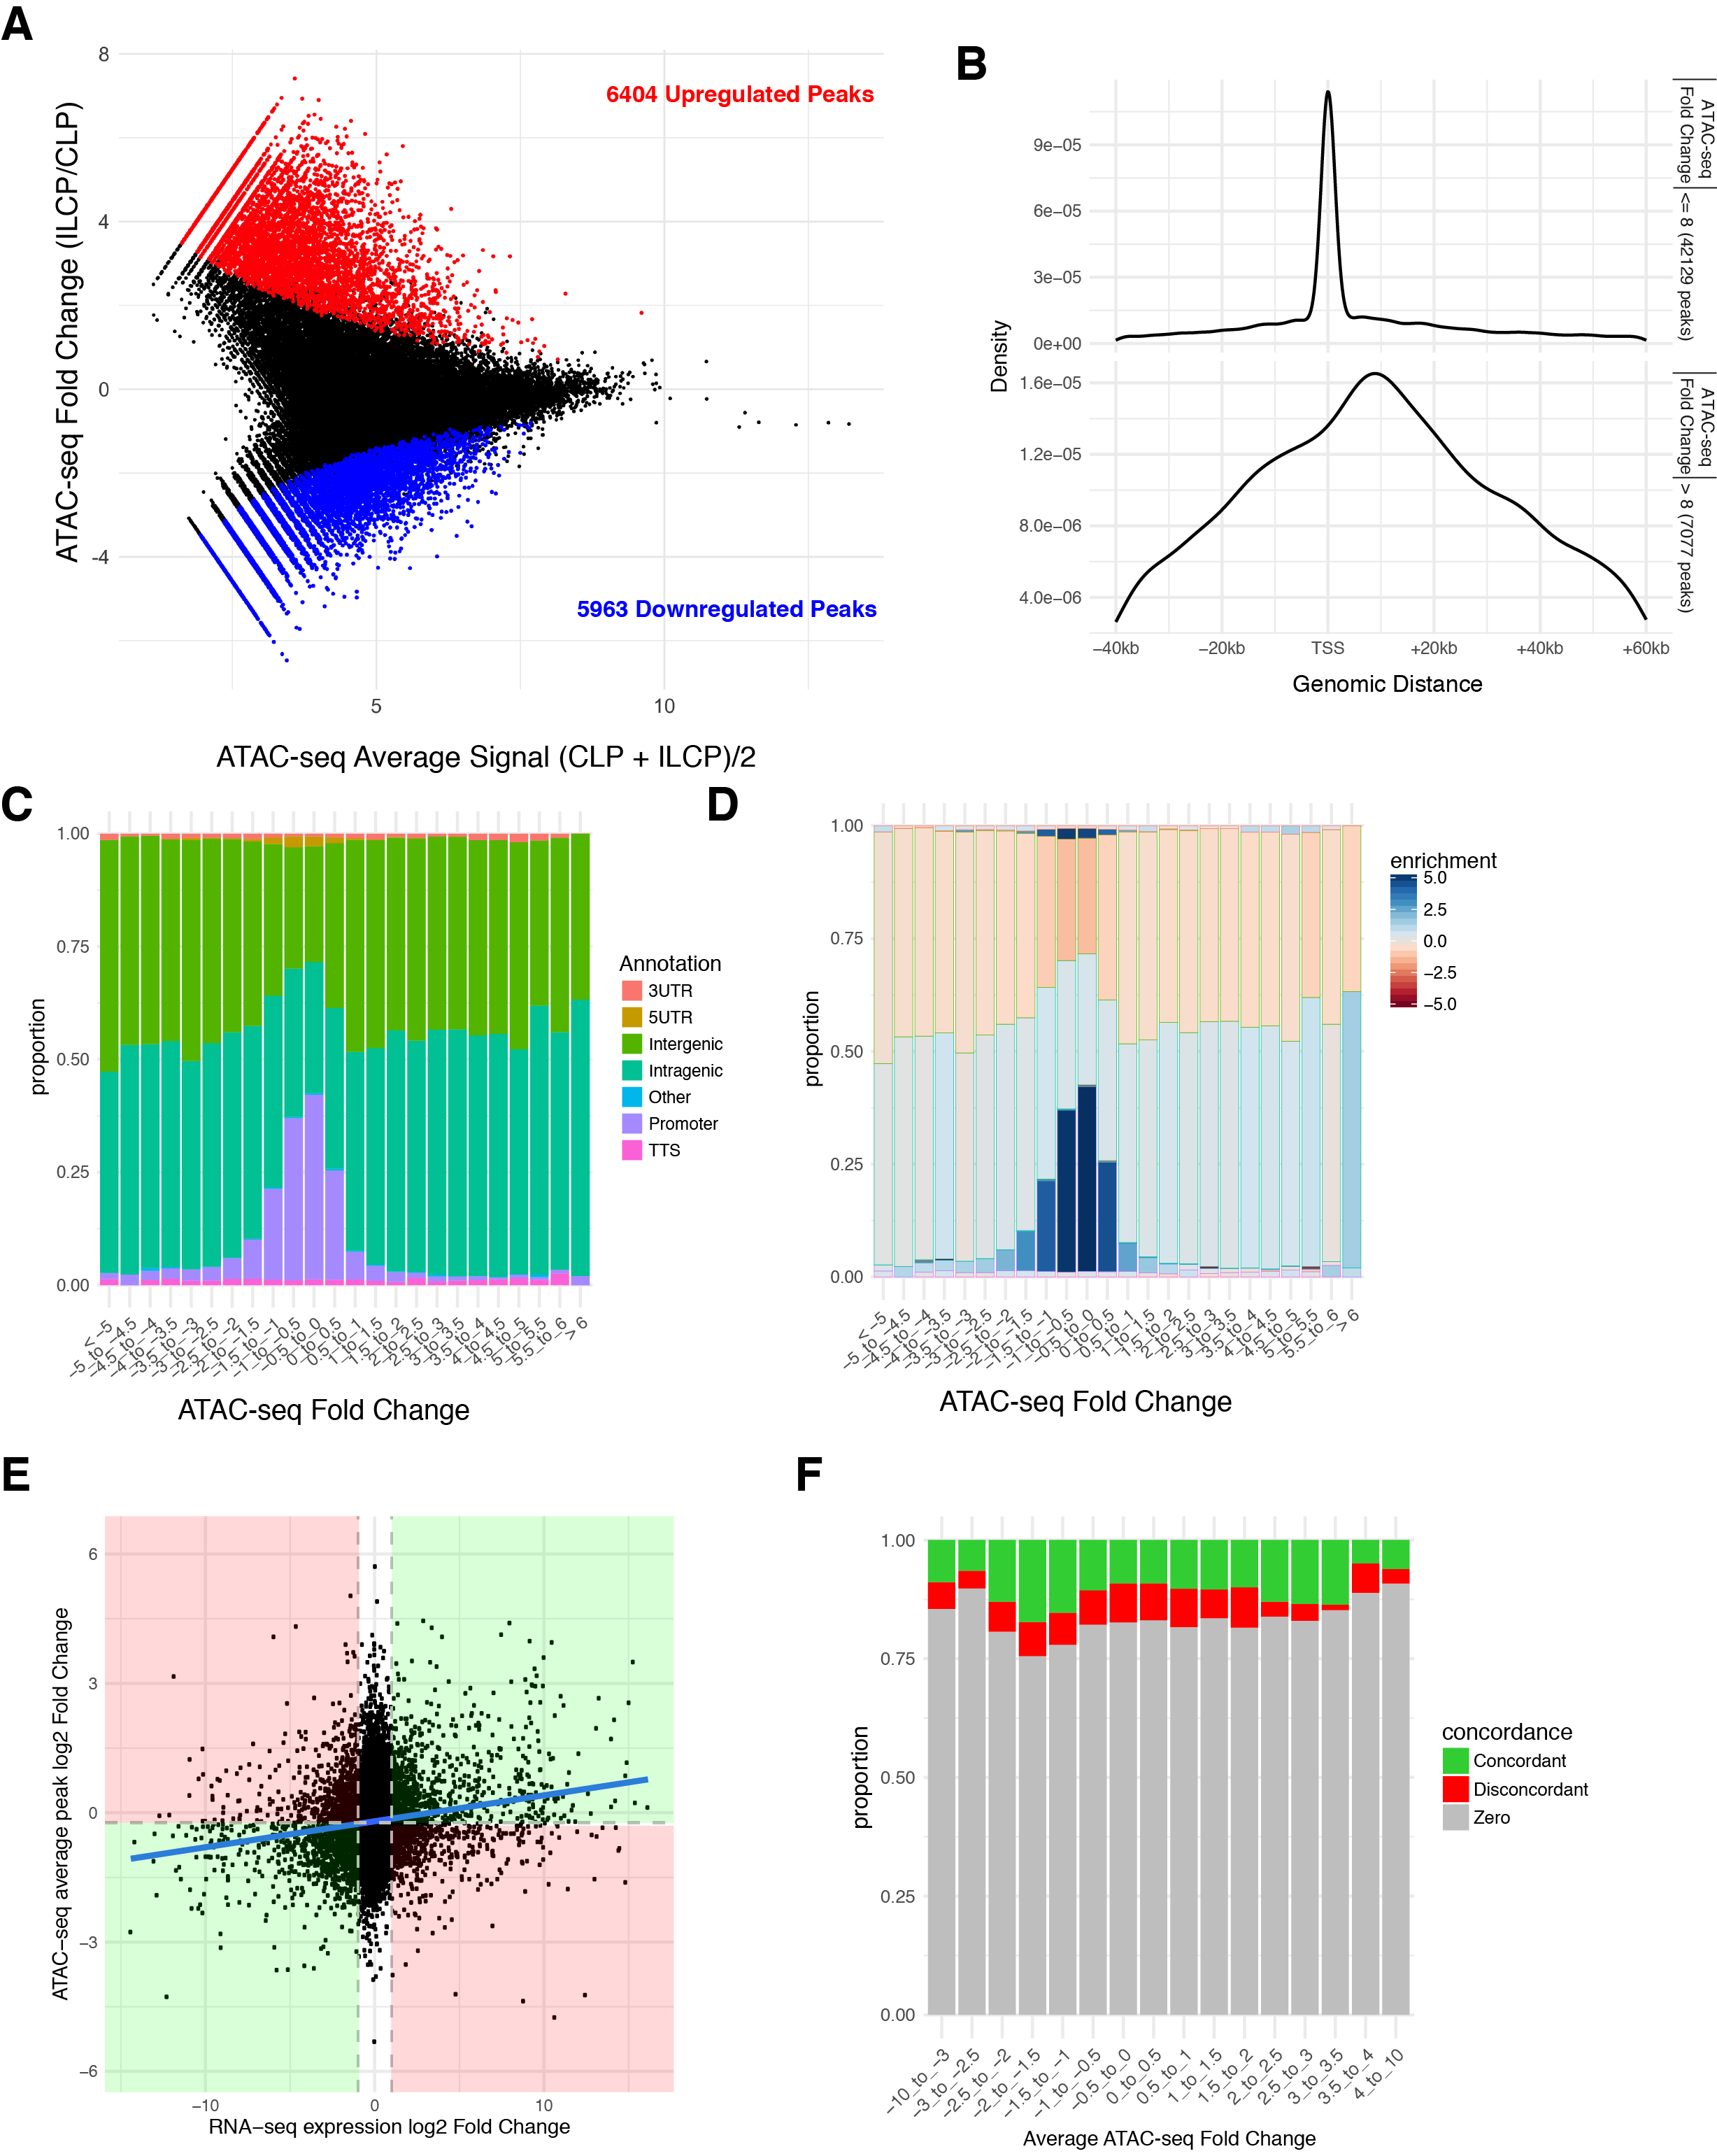
\includegraphics[width=0.85\textwidth]{figures/chapter4/Figure_3_atac_peak_locations}
\end{center}
	\caption{Enhanced distal chromatin accessibility during ILC specification.} 
	A) Increasing and decreasing regulatory elements as called by edgeR. B) Density distribution of unchanged compared to strongly changing peaks around aligned gene TSS. C) Frequency of peaks found in annotated genomic locations and D) relative enrichment of peak frequency in each genomic location. E) Correspondence between transcriptional fold change and average peak fold change in 50kb window around gene TSS. Concordant region highlighted in green and discordant region highlighted in red. Linear fit line shown in blue with Pearson correlation coefficient of 0.15. F) Proportions of genes with concordant or discordant transcriptional and chromatin dynamics grouped by average chromatin accessibility fold change.
	\label{fig:chap4_peakloc}
\end{figure}

We observe many more substantial changes in chromatin accessibility than transcriptional changes across the genome. The average fold change of regulatory elements within 50kb of a gene TSS is weakly correlated with the corresponding transcriptional change (Pearson correlation coefficient of 0.15) (Figure \ref{fig:chap4_peakloc}E). By using this local regulatory element fold change statistic to categorize genes with concordant chromatin and transcriptional changes, only $\sim$20\% have substantial transcriptional changes. Among these, most tend to be concordant with a greater bias associated with larger chromatin categories (Figure \ref{fig:chap4_peakloc}F).

This simplified analysis shows that among genes with large changes in chromatin accessibility, a small subset have concordant transcriptional changes while most remain transcriptionally unchanged. These trends point to fact that more specific attributes of peaks besides fold change and genomic location are necessary to understand how the observed chromatin changes influence gene expression.


\subsection{Motifs associated with distinct chromatin profiles}

To identify predominant regulatory factors acting in ILCP transition, we surveyed all identified regulatory elements for transcription factor motif consensus sequences. We scanned all annotated transcription factor consensus sequences from five transcription factor repositories (JASPAR, Homer, Chen, Hocomoco, Uniprobe) with FIMO to obtain locations of highly significant motif matches \cite{grant2011}. We used a hierarchical clustering strategy on motif overlap proportions to empirically group largely redundant motifs. 

While we initially expected there to be motifs correlating with opening and closing of chromatin, we were surprised to find a set of motifs distinctly associated with unchanging chromatin accessibility between CLP and ILCP. In particular, there were a number of motifs whose appearance strongly enriches for peaks with limited absolute fold change (between –1.3 to 0.7) (Figure \ref{fig:chap4_motif}A). 

%% Chapter 4 Figure 4 Motif Dynamics %%
\begin{figure}[p]
\begin{center}
	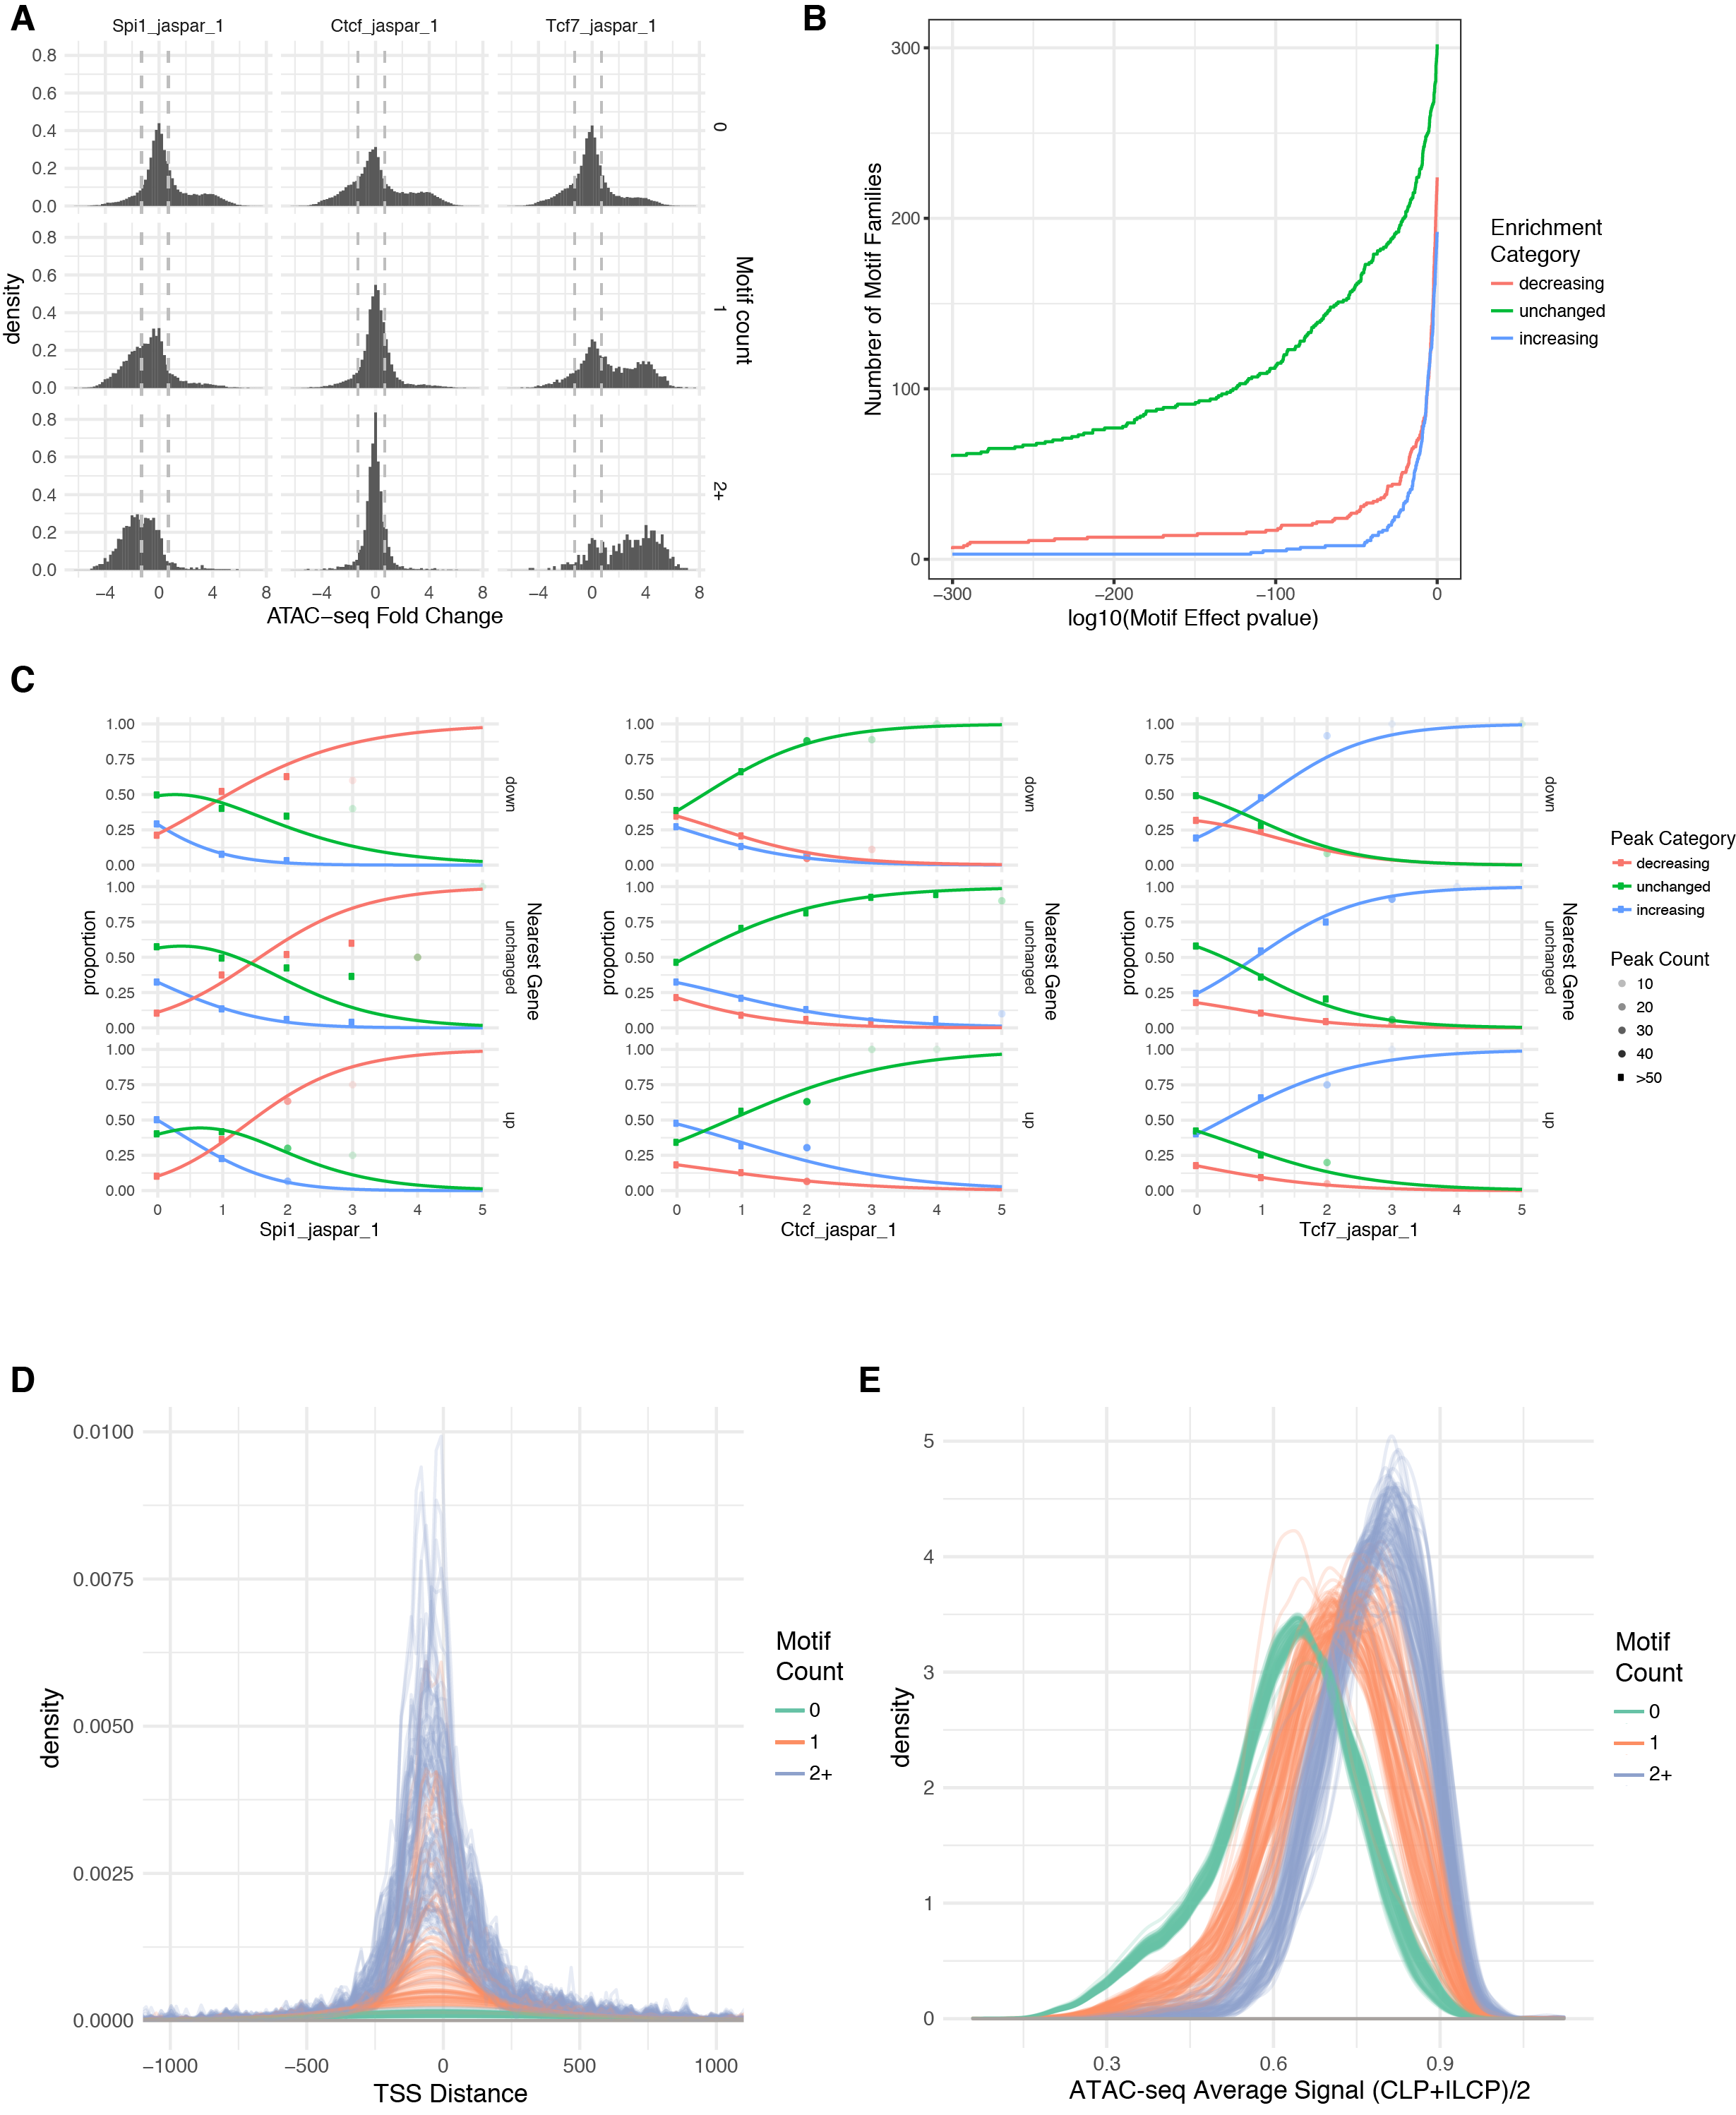
\includegraphics[width=0.95\textwidth]{figures/chapter4/Figure_4_motif_dynamics_raster}
\end{center}
	\caption{Transcription factor motifs associated with distinct chromatin profiles.} 
	A) Enrichment of delineated decreasing, unchanged and increasing regulatory elements by Spi1, Ctcf, and Tcf7, respectively. B) Number of significantly influential motif families enriching for peak group categories. C) Multinomial modeling of peak group categories. D) Motifs that enrich for unchanged regulatory elements are preferentially found in promoter regions. E) Motifs that enrich for unchanged regulatory elements are preferentially found in stable peaks with high read-counts.
	\label{fig:chap4_motif}
\end{figure}

To screen for the most influential motifs on peak dynamics, we constructed a multinomial logistic regression model that accounts for three distinct groups of peaks (increasing, unchanging, decreasing) partitioned by the previously mentioned fold change delimiters (Figure \ref{fig:chap4_motif}C). We use this model to evaluate whether the number of times a motif is found in a regulatory element significantly influences the probability that a regulatory element belongs to one of the increasing, unchanging, or decreasing sets of peaks. We found it was necessary to include the RNA expression status (upregulated, unchanged, or downregulated) of the nearest gene as confounder and interaction term, due to the previously described baseline correspondence between transcriptional changes and local chromatin openness. For each motif, we fit this multinomial model and calculated the significance of the motif coefficients from type I ANOVA with interaction. We Benjamini-Hochberg corrected the full set of significance values to associate motifs with corresponding false discovery rates (FDRs). 

Generally, many motifs were associated with significant multinomial regression models, likely due to the large number of predictive peaks in dataset. There were slightly more motifs that tend to enrich for increasing regulatory elements than those that enrich for decreasing regulatory elements, but by far most motifs actually enrich for the empirically defined set of unchanged regulatory elements (Figure \ref{fig:chap4_motif}B). The group of motifs that enrich for unchanged peaks is comprised of transcription factors with seemingly mixed functional origins. Notably, this group includes CTCF, an architectural protein responsible for defining chromatin looping structures and organization. We also observed a number of E2F family transcription factors as well as Myc, which have roles in cell cycle progression. Other transcription factor families found notably bind GC-rich motif sequences, including SP, EGR, KLF, and AP-2. Collectively, we observed that the presence of these motifs particularly enrich for regulatory elements in promoter regions (Figure \ref{fig:chap4_motif}D), and also for regulatory elements with high average read-count in CLP and ILCP (Figure \ref{fig:chap4_motif}E), which corroborates that these motifs specifically enrich for persistent regulatory features. 

%% Chapter 4 Figure 5 Enrichment Results %%
\begin{figure}[p]
\begin{center}
	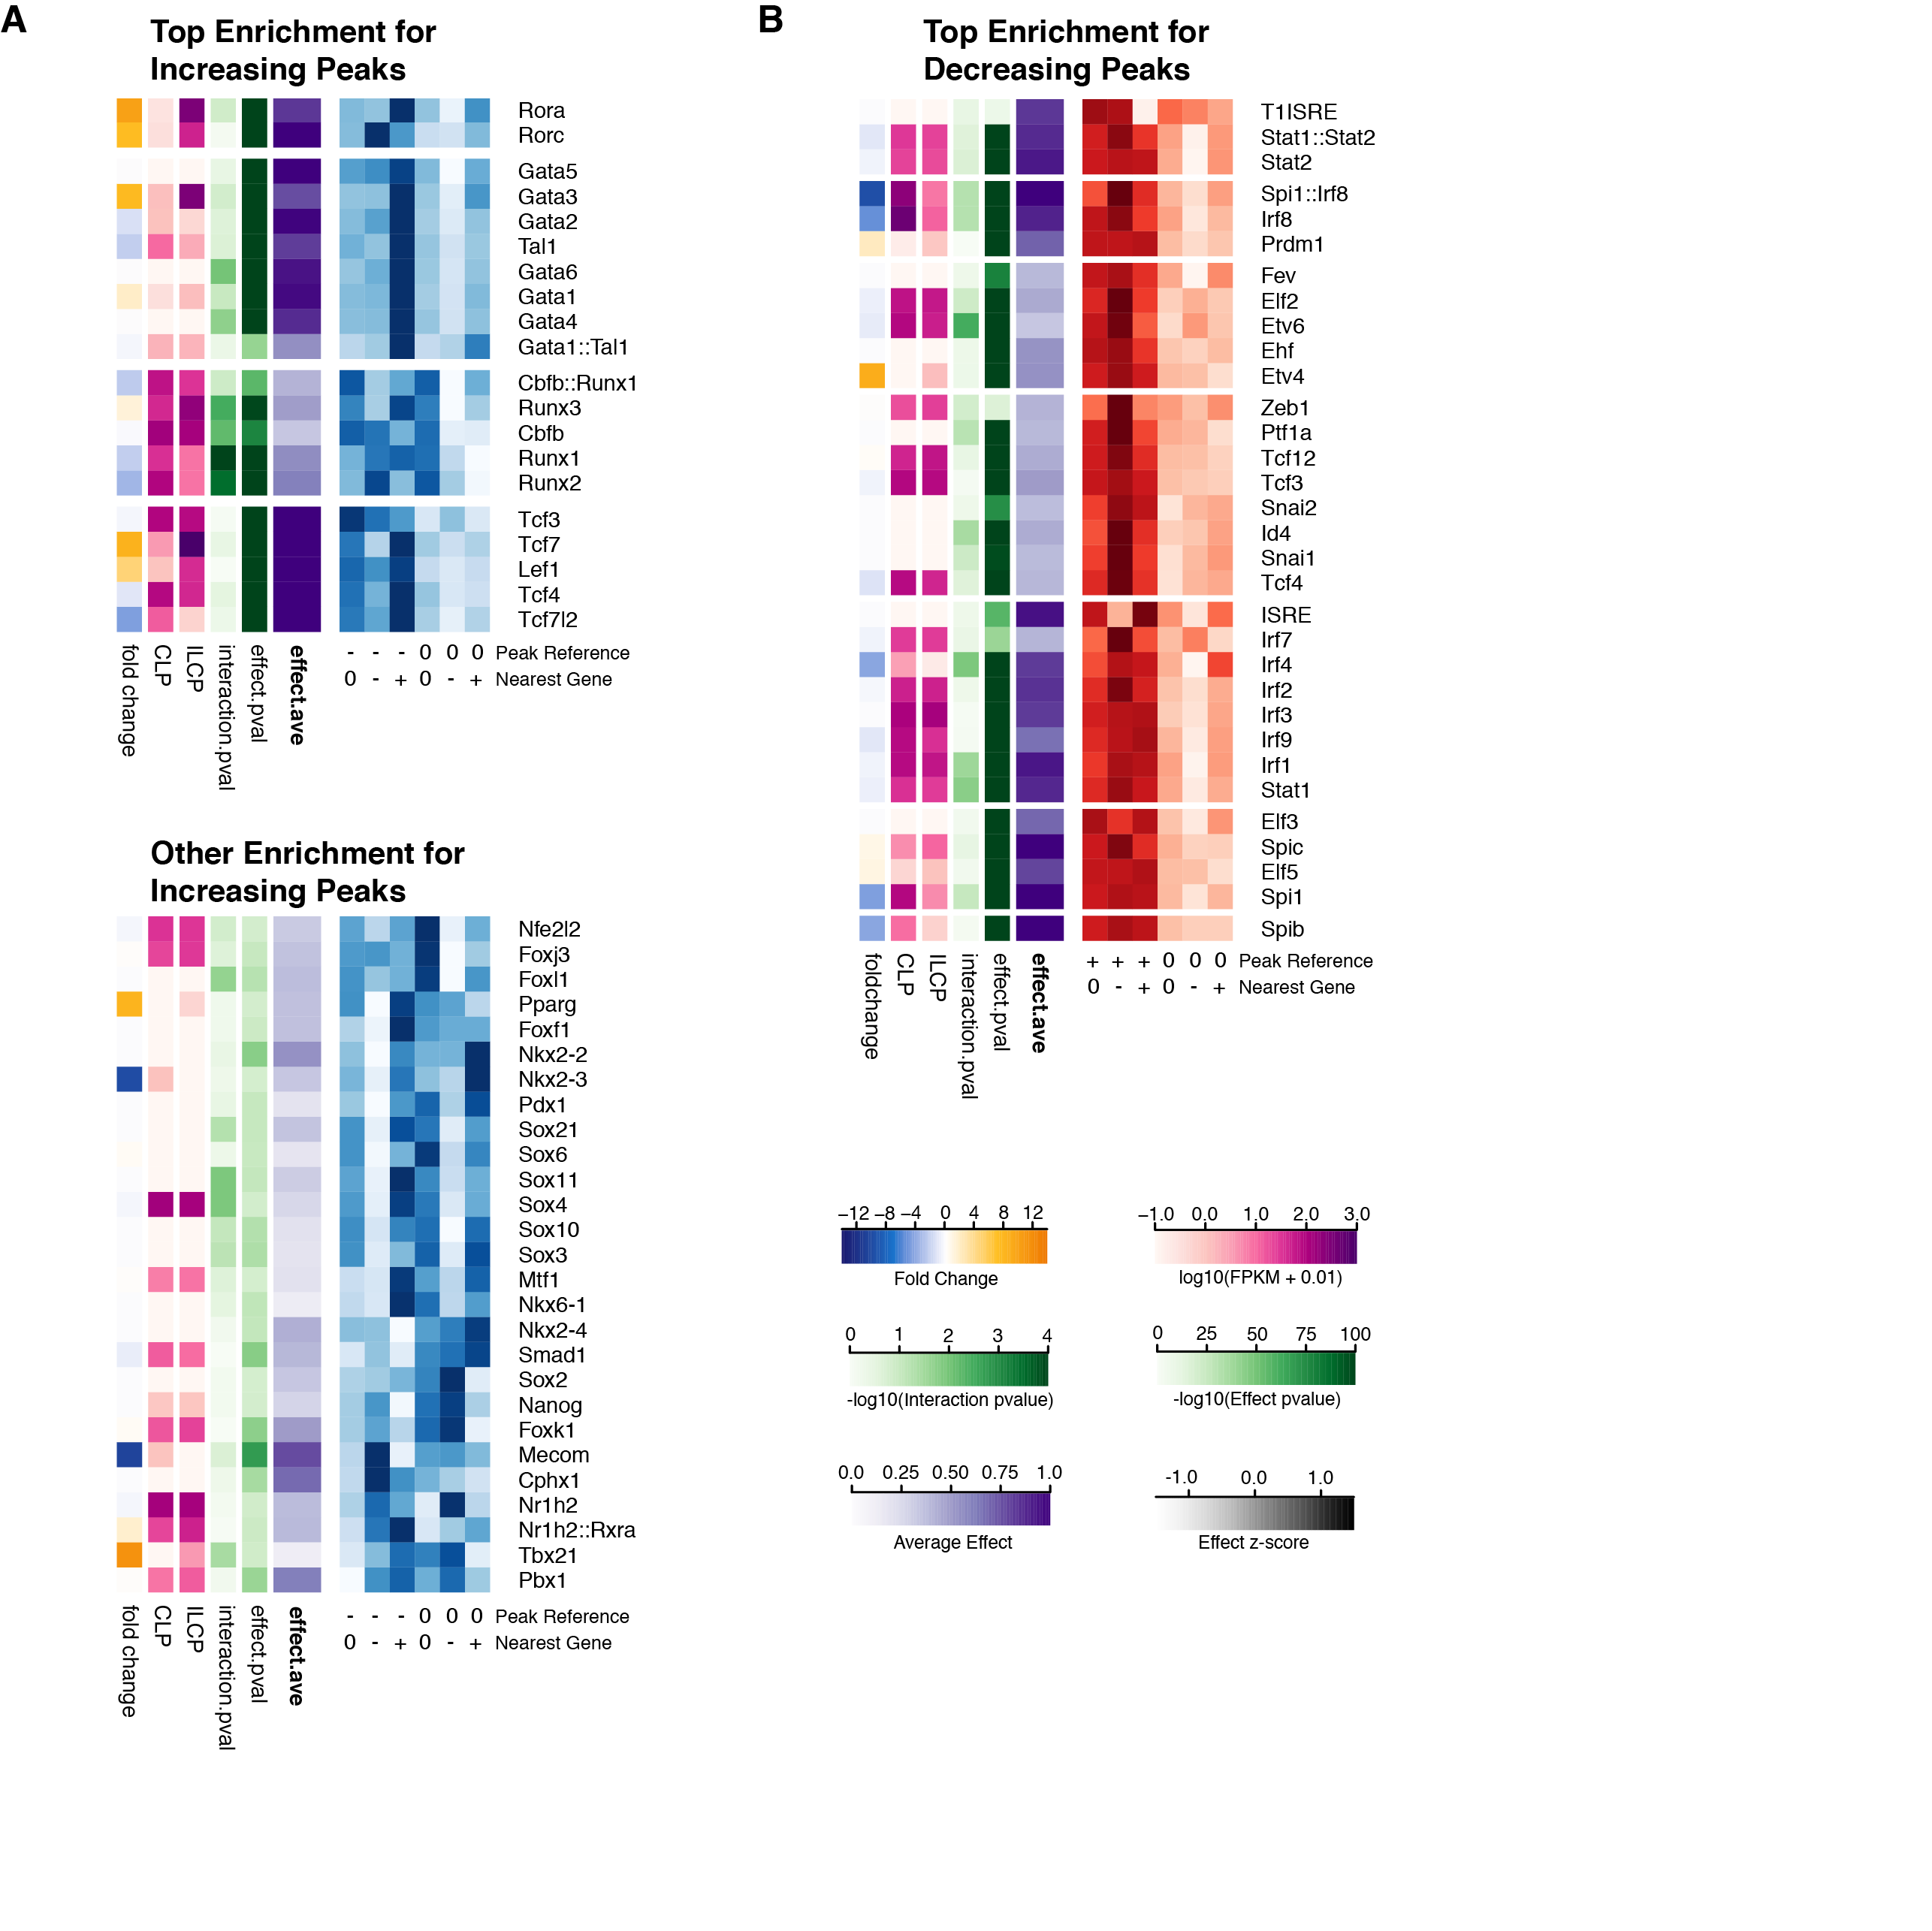
\includegraphics[width=\textwidth]{figures/chapter4/Figure_5_enrichment_results}
\end{center}
	\caption{Transcription factor motifs enrich for changing chromatin.} 
	A) Top motifs that enrich for increasing regulatory elements. B) Top motifs that enrich for decreasing regulatory elements. 
	\label{fig:chap4_enrich}
\end{figure}

Among all motif groups that significantly enrich for increasing regulatory elements, the TCF, ROR, GATA and RUNX motif families stand out with exceptionally large influences on peak dynamics (Figure \ref{fig:chap4_enrich}A). Each of these families has multiple individual motif members with significance levels far beyond all others surveyed. Motifs affiliated with the TCF family are among the most strongly enriching with an average multinomial model coefficient of 1.5, implying that each TCF motif enhances the odds of belonging to the set of increasing peaks by more than a factor of 4. We anticipate this strong influence on peak dynamics is driven by Tcf7, given that Tcf7 transcription is the most significantly upregulated of any transcription factor. Interestingly, both ROR family members identified, nuclear receptors \RORa{} and \RORgt, have integral roles in ILC development and are substantially upregulated at the ILCP stage. As a master regulator of both ILC3 and LTi lineages, \RORgt{} has spotted transcription prior to differentiation in ILCP. While defective \RORa{} specifically impacts ILC2 differentiation, \RORa{} is widely expressed in most ILCP after induction of PLZF and in peripheral ILCs and LTi. Among GATA family members, we anticipate enrichment of increasing peaks to be driven by Gata3, master regulator of the ILC2 lineage, since Gata3 is also widely expressed in ILCP prior to differentiation and impacts multiple ILC lineages when perturbed. These ROR and GATA family results in particular highlight how lineage specific transcription factors could play early regulatory roles prior to ILC differentiation. Among RUNX family members, both Runx1 and Runx3 have transcriptional dynamics that could fit with early regulatory roles. In single-cell study, Runx1 was observed to have a transient transcriptional peak prior to PLZF induction. Recently, it has been found that Runx3 is expressed at the ILCP stage and is essential for the development of ILC1s and ILC3s. While TCF, ROR and GATA family members have relatively equal enrichment rates despite the transcriptional dynamics of the nearest gene, RUNX family members interestingly have significantly altered effect coefficients depending on these categories of transcriptional change. Runx1 in particular tends to have enhanced enrichment for increasing peaks near downregulated genes. The predominant four motif families whose presence enriches for increasing peaks recapitulate known influencers in ILC development, but point to their specific association with new regulatory elements found in ILCP.

We detected a number of motifs in addition to these relatively known factors that specifically enrich for increasing regulatory elements (Figure \ref{fig:chap4_enrich}A). Interestingly, these include Tbx21, master regulator of the ILC1 lineage, and SOX family motifs, of which Sox4 is transcriptionally induced just prior to the ILCP. We also found Nanog and Sox2, key pluripotency regulators in embryonic stem cells, as well as a number of motifs with reported roles in regulating hematopoietic stem cell differentiation, such as FOX family genes, Nfe2l2 (or Nrf2), Mecom (or Evi1), and Pbx1. As a mediator of Notch pathway signaling, Nrf2 could be of particular interest given the necessary role of Notch signaling in early ILC specification. Finally, we found Nr1h2 and Pparg, which are known to interact with retinoid receptors. Further investigation is required to determine if some of these factors have roles in ILC development or if their genomic locations are similarly regulated by other ILC specific factors.

Most of the motifs that significantly enrich for decreasing peaks are affiliated with B cell development (Figure \ref{fig:chap4_enrich}B). Two motifs that most strongly enriched for decreasing peaks include Spi1 (or PU.1) and Spib, complementary ETS family transcription factors associated with the B cell lineage. We also found IRF family members that strongly enriched for decreasing peaks, which are known to participate in B cell fate decisions in concert with Spi1. Both Spi1 and Irf8 in particular were substantially transcriptionally downregulated, suggesting decreasing regulatory elements could be directly explained by decreased occupancy of these factors. Interestingly, we also found a motif family that includes Tcf3 (or E2A) that enriches for decreasing peaks. While Tcf3 was not substantially transcriptionally downregulated, Tcf3 is expressed in both CLP and ILCP and is known for mutual antagonism with (the strongly upregulated) ILC lineage-specific factor Id2. While Ebf1 motifs trended towards enrichment for against increasing peaks, the effect sizes were not substantial enough to be strongly significant (not shown). This is somewhat surprising given the relatively strong transcriptional downregulation of Ebf1 and its established role in early B cell development, and highlights stronger regulatory influence of earlier lymphoid factors at the CLP stage. 

\section{DISCUSSION}

In this study, we directly compare transcriptomic and epigenomic information to better describe the global regulatory changes that occur during ILC specification. Our genome-wide transcriptional characterization of the transition between CLP and ILCP highlights predominant transcriptional changes that define the ILCP developmental stage, including ILC specific transcriptional regulators and surface markers. By surveying the ILCP, we present a comprehensive transcriptional profile of the stage committed to the ILC lineages, but just prior to extensive lineage differentiation. 

Given the intricate set of successive transcriptional changes that occurs throughout early ILC specification, this survey of changes occurring at ILCP stage reveals useful markers that can tease out finer stages of development. For instance, one of the most highly upregulated surface markers in ILCP that we identified, Pdcd1, has been shown to be an effective proxy for PLZF expression in ILC progenitor cells, allowing for the isolation of the ILCP without specific reporter mice \cite{seillet2016,yu2016}. We anticipate that some of the uncharacterized transcription factors and surface markers that we found associated with the ILCP could help distinguish ILC progenitor stages or be associated with branching of specific ILC lineages. 

The low cell number requirements for ATAC-seq enabled the survey of chromatin accessibility for the rare ILC precursor population. While the ILCP has a more restricted developmental potential than the CLP, we generally observed more opening regulatory enhancers with larger fold-changes than closing enhancers at the ILCP stage. Consistent with other studies, we found that the most significantly changing regulatory enhancers tend to be distal rather than proximal to gene transcription start sites. More broadly across hematopoiesis, distal enhancers are a more reliable predictor of cell identity than proximal enhancers or even transcriptional profiles \cite{corces2016}. In the comparison of chromatin accessibility between differentiated ILC effectors, common regulatory enhancers tend to be found in promoter regions while variable regulatory enhancers that distinguish different ILC lineages are found in distal genomic locations \cite{shih2016}. We also observed that changes in chromatin accessibility surrounding gene TSS tend to be more prevalent than corresponding changes in gene transcription. Further study is required to determine if these widespread chromatin accessibility changes can be assigned functional roles in differentiated ILCs or other lineages. 

By examining the distribution of transcription factor motifs among regulatory elements, we were able to learn more specific information about transcriptional regulation occurring during ILC specification. We demonstrate through statistical modeling that the presence of motif sequences in regulatory regions is highly predictive of changes in chromatin accessibility in those regions. Moreover, the models demonstrate the direct relationship between motif count and accessibility. This is compelling since we can identify these strong associations between motifs and chromatin regulation without needing to restrict our evaluation to true binding events, as could be measured by CHIP-seq for instance. This affords us the ability to scan and evaluate the influence of hundreds of motifs systematically, which would be prohibitively expensive to perform experimentally. Granted, we are precluded from evaluating motifs without well-established motif consensus sequences. Still, from this large set of motif comparisons, we identified the most influential set of motifs that should be prioritized for further investigation.

In specifying a logistic regression model for examining the association between motif presence and chromatin accessibility, we uncovered a set of motifs that enrich for unchanging regulatory elements that we did not anticipate. By considering unchanging ATAC-seq peaks as a distinct group from increasing or decreasing peaks, we could isolate a large number of motifs with roles that are likely separate from lineage specification. While it is difficult to provide a collective interpretation for this set of motifs, it notably includes the architectural protein CTCF, cell cycle regulators such as E2A, and generic transcriptional promoters of development and proliferation. We also noticed that a number of these motifs bind GC-rich sequences, which leads us to speculate that they might be associated with CpG islands found in a large portion (40\%) of mammalian promoter regions. Given that the CLP and ILCP populations that we analyzed are both progenitor populations, it is not clear if the large number of developmental factors found in this group is specific to progenitor cells or could be as extensively observed in differentiated cells as well. The different types of motifs found in this group illustrate the diverse functional categories of regulatory enhancers that are simultaneously surveyed in chromatin profiling studies.

Our statistical modeling also highlighted the predominant enrichment for opening chromatin by the TCF, ROR, GATA and RUNX motif families. Of all TCF family members, Tcf7 is highly expressed at the ILCP stage and required for development of all known ILC subsets \cite{yang2015,mielke2013,yang2013}. Similarly, Gata3 of the GATA family is highly expressed at the ILCP stage and required for development of all ILC subsets and LTi \cite{yagi2014}. Multiple members of the RUNX family could be acting at the ILCP stage. Runx3 expression is particularly affiliated with differentiated ILC1 and ILC3 lineages but is also present in ILCP. From our single-cell studies, Runx1 appears to have peak expression just prior to the upregulation of PLZF and could be acting earlier in ILC development. We also note that we observed upregulation of Zbtb7b (or Th-POK), an important T cell differentiation factor that also belongs to the RUNX family. Two members of the ROR family, \RORa{} and \RORgt, have necessary roles in promoting ILC2 and ILC3 development, respectively. While all of these highlighted motif families contain factors known to influence ILC development, our findings point to their specific association with remodeled chromatin in the ILCP stage. Given the increased transcription of regulatory factors belonging to each of these four motif families, the most direct interpretation for their enrichment of opening chromatin in ILCP is increased occupancy in these new regulatory regions.

Besides just indicating which transcription factors are associated with remodeled chromatin, our statistical modeling provides an initial indication of how these factors might be acting in regulatory elements. Generally, the relatively consistent influence of motif presence on peak dynamics regardless of the transcriptional dynamics of the nearest gene suggests that these regulatory factors can have either activating or inhibitory roles depending on context. For instance, Tcf7 motifs widely appear preferentially in opening chromatin near both upregulated and downregulated genes. In fact, Tcf7 motifs tend to appear more frequently near downregulated genes (data not shown). Interestingly, another study found that perturbation of Tcf7 in early ILC progenitors results in upregulation of B cell affiliated genes, illustrating both the inhibitory role of Tcf7 and regulation of competing lineages \cite{seillet2016}. 

Collectively, our study characterizes the genome-wide set of transcriptional and epigenetic features coincident with ILC specification. While uncovering both known and novel transcriptional regulators, our statistical modeling provides further insight into the potentially important roles these factors have in ILC development. 

\section{METHODS}

\textit{RNA-seq data acquisition} Pooled samples of CLP and ILCP with unpaired 50bp reads were sequenced with Illumina Hi-seq. Read alignment was performed with bowtie2 and transcript quantification with eXpress. Without biological replicates for measured cell types, we could not perform traditional differential expression analysis and calculate the significance of expression changes as we cannot estimate expression variance. To obtain ranking of transcriptional changes, we performed edgeR differential expression analysis with a fixed biological coefficient of variation suggested in edgeR manual. We then determined the significance ranking with these estimated significance values. We anticipate this procedure yields a more realistic prioritization than fold change ordering since it incorporates read-count information. Since the overall significance scale returned by this procedure arbitrarily depends on the chosen biological coefficient of variation, we chose a significance cutoff that yielded 201 upregulated and 164 downregulated genes. Gene set enrichment analysis was performed using the desktop java application based on the fixed ordering of transcriptional change just described using an unweighted statistic. Gene set size was limited to 300 to filter very large gene set annotations. 
\\
\textit{ATAC-seq data acquisition} Three CLP and two ILCp replicate samples with paired 50bp reads were sequenced by Illumina Hi-seq. Read alignment was performed with bowtie2. After alignment, read locations were shifted according to the tn5 transposase strand bias (+4bp for reads on the  + strand, and -–5bp for reads on the -– strand). Peak features were called for each sample separately using MACS2 at FDR 0.01 with 5 allowed duplicates at any position. The complete peak set was subsequently filtered to only include peaks called in at least all CLP or all ILCP samples. Differential read-count analysis was performed using the edgeR option in the DiffBind R package. Fold change thresholds for demarcating increasing, decreasing, or unchanged groups of ATAC-seq peaks were determined empirically through observation of the enriched set of unchanged peaks by particular motifs. Sp4 in particular was widely found in peaks and the fold change boundaries were based on the unchanged peak subset strongly enriched by Sp4. 
\\
\textit{Motif database scanning} Motif consensus sequences were aggregated from the JASPAR, Homer, Chen, Hocomoco, and Uniprobe transcription factor repositories. If possible, motifs were assigned the nearest mouse homolog for interpretation and to assign expression values. Motif sequences were scanned across all regulatory element regions as called above with FIMO from the MEME suite \cite{grant2011} with a p-value threshold of 1e-4. To account for redundant motif entries between and within databases, we defined an empirical grouping of motif families based on overlap. For each pair of motifs, we calculated the proportion of occurrences where the two motifs were found in overlapping locations. To define motif families, we then performed hierarchical clustering on this proportion overlap data, using a complete linkage criterion that corresponds to at least 20\% overlap required among all family members. 
\\
\textit{Multinomial logistic model} A multinomial logistic regression model was used to test for peak group (increasing, decreasing, unchanged) enrichment by motif presence. The following system of equations was fit for each tested motif: 
\begin{align}
	\log{\left(\frac{P_{increasing}}{P_{decreasing}}\right)} &= C + C_{RNA} + C_M \cdot MOTIF + C_{M,RNA} \cdot MOTIF \\
	\log{\left(\frac{P_{increasing}}{P_{unchanged}}\right)} &= D + D_{RNA} + D_M \cdot MOTIF + D_{M,RNA} \cdot MOTIF
\end{align}

where $P_{group}$ is the probability that the regulatory element belongs to the labeled peak group, $RNA$ is the transcriptional status of nearest gene (upregulated, downregulated, unchanged), and $MOTIF$ is the number of motif sequences found in the regulatory element. For motifs in which some multinomial categories did not have a sufficient number of peaks, a set of peaks were pre-populated to avoid instabilities that derive from fitting 0 proportions in multinomial regression. Specifically, the complete set of peaks with all possible combinations of peak group, $RNA$, and 0 and 1 $MOTIF$ numbers were included when pre-populating. We evaluated model significance with type I ANOVA, which successively tests for significant attribution of the total sum of squares ($SS$) to the components $SS(RNA)$, $SS(MOTIF | RNA)$, and $SS(MOTIF*RNA | RNA, MOTIF)$. We refer to the last two corresponding p-values as the motif effect p-value and the interaction p-value, respectively. To identify the strongest enrichment group for each motif, we compare coefficients from each of three possible reference group directions and choose the one with the largest absolute coefficients. We calculate the weighted average of motif effect coefficients, with weights defined as inverse estimated variance, for the overall motif effect measure. Logistic regression models were fit using the nnet package in R. 

%%% END CHAPTER 4 CHROMATIN ACCESSIBILITY %%%


